% SPDX-FileCopyrightInfo: Copyright © DuMux Project contributors, see AUTHORS.md in root folder
% SPDX-License-Identifier: CC-BY-4.0
%
% LaTeX source for multi-phase image
% compile to svg with poppler by running
%    pdflatex multiphase_processes.tex
%    pdftocairo -svg multiphase_processes.pdf
\documentclass[crop,tikz]{standalone}
\usetikzlibrary{decorations}
\usetikzlibrary{decorations.pathmorphing}
\begin{document}
  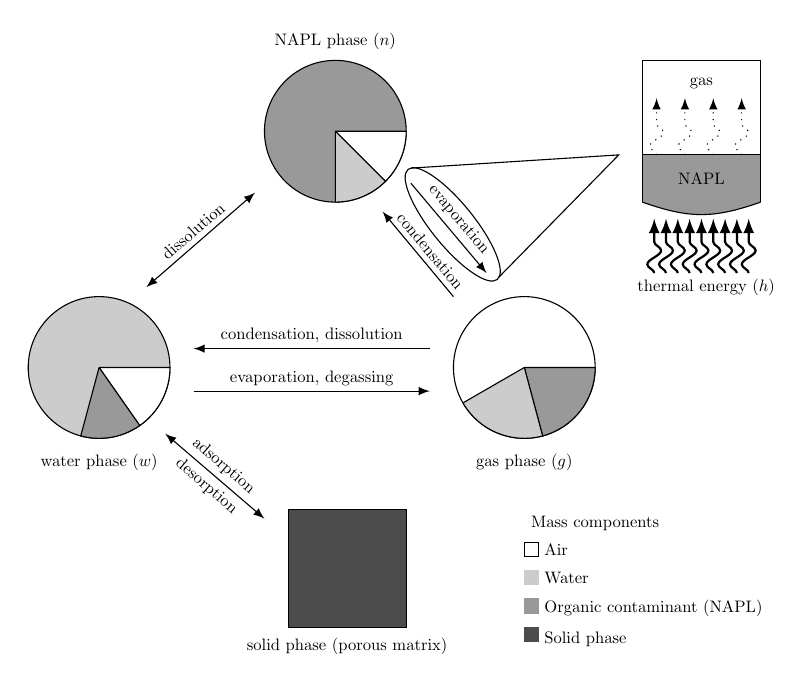
\begin{tikzpicture} [>=latex,scale=0.6, every node/.style={transform shape}]
    % Ellipse 1 solid
    \coordinate (A) at (1,-0.5);
    \draw [fill=black!70](A) rectangle(3.5,2) node at(2.25,-0.9) {solid phase (porous matrix)};
    % Ellipse 2 water
    \coordinate (B) at (-3,5);
    \draw [fill=black!20](B) circle(1.5cm);
    \node [yshift=5mm]at(-3,2.5){water phase $(w)$};
    \draw[fill=white] (B)--+(1.5,0)arc(0:-55:1.5cm)--(B);
    \draw[fill=black!40] (B)--+(-55:1.5cm)arc(-55:-105:1.5cm)--(B);
    % Ellipse 3 gas
    \coordinate (C) at (6,5);
    \draw [](C) circle (1.5cm);
    \node[yshift=5mm]at(6,2.5){gas phase $(g)$};
    \draw [fill=black!40](C)--+(1.5,0)arc(0:-75:1.5cm)--(C);
    \draw [fill=black!20] (C)--+(-75:1.5cm)arc(-75:-150:1.5cm)--(C);
    % Ellipse 4 napl
    \coordinate (D) at (2,10);
    \draw [fill=black!40](D) circle (1.5cm);
    \node[yshift=5mm]at(2,11.4){NAPL phase $(n)$};
    \draw [fill=white](D)--+(1.5,0)arc(0:-45:1.5cm)--(D);
    \draw [fill=black!20] (D)--+(0,-1.5)arc(-90:-45:1.5cm)--(D);
    % arrows
    %A-B
      \draw [<->,white](0.5,1.8)--(-1.6,3.6) node[black,above,sloped,pos=0.5]{adsorption};
      \draw [<->](0.5,1.8)--(-1.6,3.6) node[below,sloped,pos=0.5]{desorption};
    %B-C
      \draw[<-](-1,5.4)--(4,5.4)node[above,sloped,pos=0.5]{condensation, dissolution};
      \draw[->](-1,4.5)--(4,4.5)node[above,sloped,pos=0.5]{evaporation, degassing};
    %B-D
      \draw[<->](-2,6.7)--(0.3,8.7)node[above,sloped,pos=0.5]{dissolution};
    %D-C
      \draw[->](3.6,8.9)--(5.2,7)node[above,sloped,pos=0.5]{evaporation};
      \draw[rotate around={-51:(4,6.8)}](3.35,7.95) ellipse (1.5cm and 0.45cm);  %Ellipse um evaporation
      \draw (3.6,9.22)--(8,9.5)--(5.45,6.9);
      \draw[<-](3,8.3)--(4.5,6.5)node[above,sloped,pos=0.55]{condensation};
    % thermal energy
    \filldraw [black!40](8.5,9.5)rectangle(11,8.5);
    \draw (8.5,9.5)rectangle(11,11.5);
    \draw (8.5,9.5)--(8.5,8.5);
    \draw (11,9.5)--(11,8.5);
    \draw [decorate,decoration={bent,aspect=0.4,amplitude=6},fill=black!40](11,8.5)--(8.5,8.5);
    \foreach \x in {8.75,9,...,10.8}
    \draw [->,decorate,decoration={snake,post length=2mm},thick](\x,7)--(\x,8.15);
    \foreach \x in {8.8,9.4,10,10.6}
    \draw [->,dotted,decorate,decoration={snake,post length=2mm}](\x,9.5)--(\x,10.7);
    \node at(9.75,11){gas};
    \node at(9.75,9){NAPL};
    \node at(9.85,6.7){thermal energy $(h)$};
    % legende
    \node at (7.5,1.7){Mass components};
    \draw[](6,1)rectangle +(0.3,0.3) node at(6.3,1.15) [right]{Air};
    \filldraw[black!20](6,0.4) rectangle +(0.3,0.3) node at (6.3,0.55)[black,right]{Water};
    \filldraw[black!40](6,-0.2) rectangle +(0.3,0.3) node at (6.3,-0.1)[right,black]{Organic contaminant (NAPL)};
    \filldraw[black!70](6,-0.8) rectangle +(0.3,0.3) node at (6.3,-0.75)[right,black]{Solid phase};
  \end{tikzpicture}
\end{document}
